\chapter{Continuous Random Variables}\label{chap:Continuous-Random-Variables}

In the previous chapter, we saw how a discrete random variable assumes countable values. If we want a random variable to take on uncountably many values, then we must turn to continuous random variables instead.

\begin{definition}\label{def:CRV}
    A \vocab{continuous random variable} is a random variable that can take on any value in a given interval.
\end{definition}

Since the value of a continuous random variable is uncountable, it can only take on an interval of values, not a specific value.

An example of continuous random variables is the volume of beverage (in ml) in a 500 ml bottle ($100 \leq X \leq 200$, $200 \leq X \leq 300$, etc.)

\section{Discrete to Continuous}

In the previous chapter, we saw how we could represent the probability distribution of a discrete random variable using a table. For instance, the probability distribution of the outcome of a single throw of a 6-sided dice is given by the following table:

\begin{center}
    \begin{tabular}{|r|c|c|c|c|c|c|}
        \hline
        $x$ & 1 & 2 & 3 & 4 & 5 & 6 \\ \hline
        $\P{X = x}$ & $\frac16$ & $\frac16$ & $\frac16$ & $\frac16$ & $\frac16$ & $\frac16$ \\ \hline
    \end{tabular}
\end{center}

We can try to specify the distribution of a continuous random variable in the same way. Consider the lengths, in millimetres, of 50 leaves that have fallen from a particular tree. We can illustrate the distribution of the lengths using a histogram:

\begin{figure}[H]
    \centering
    \tikzsetnextfilename{421}
    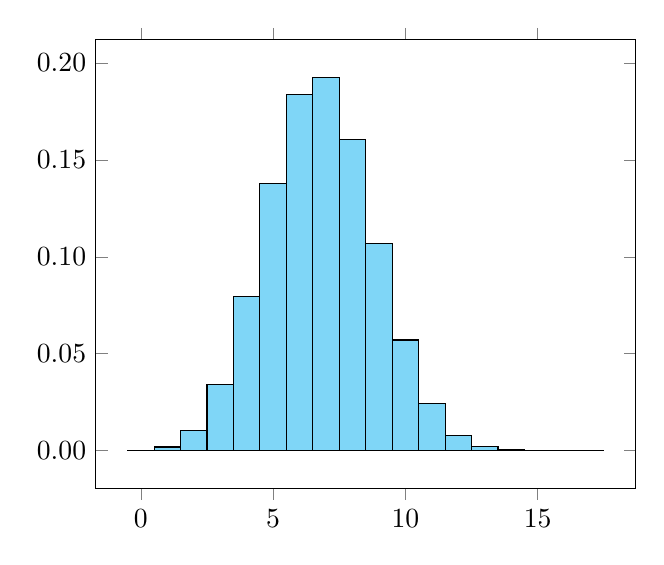
\begin{tikzpicture}[
        declare function={binom(\k,\n,\p)=\n!/(\k!*(\n-\k)!)*\p^\k*(1-\p)^(\n-\k);}
    ]
    \begin{axis}[
        samples at={0,...,17},
        yticklabel style={
            /pgf/number format/fixed,
            /pgf/number format/fixed zerofill,
            /pgf/number format/precision=2
        },
        legend style={at={(0.5, -0.15)},anchor=north},
        ybar=0pt, bar width=1
    ]
    \addplot [fill=cyan, fill opacity=0.5] {binom(x,17,0.4)};
    \end{axis}
    \end{tikzpicture}
    \caption{A histogram of the lengths of leaves.}
\end{figure}

Here, the vertical axis represents the frequency density of lengths in a particular interval, hence the total area of the histogram is 1. This property also allows us to find the probability that a length is in a given interval: simply sum up the area of the rectangles in the given interval. 

Notice that if we want the probability of a certain length, e.g. $L = 6.3$ cm, the answer would be zero. Though it is theoretically possible for $L$ to be $6.3$ cm exactly (i.e. $6.30000\dots$), the probability is actually zero. This means that \[\P{6 < L < 7} = \P{6 \leq L < 7} = \P{6 < L \leq 7} = \P{6 \leq L \leq 7}.\] That is, whether we include the bounds of the interval does not affect the probability that $L$ falls within the interval.

The probabilities calculated from the histogram could be used to model the length of a tree leaf. However, the model is crude, because of the limited amount of data, and the small number of classes in which the leaves are grouped into, resulting in the ``steps'' in the histogram.

The model could be further refined by repeating the process of collecting more data and reducing the class width. If this process were to be continued indefinitely, then the outline of the histogram would become a smooth curve:

\begin{figure}[H]\tikzsetnextfilename{425}
    \centering
    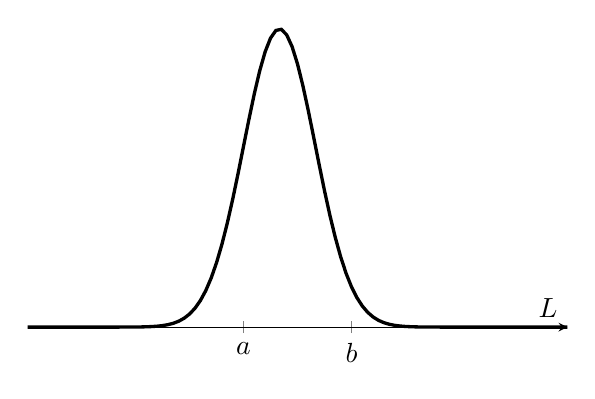
\begin{tikzpicture}[trim axis left, trim axis right]
        \begin{axis}[
            domain = 0:15,
            ymin = -0.1,
            ymax = 0.5,
            samples = 101,
            axis x line=middle,
            axis y line=none,
            xtick = {6, 9},
            xticklabels = {$a$, $b$},
            xlabel = {$L$},
            legend cell align={left},
            legend pos=outer north east,
            ]
            \addplot[black, very thick] {1/sqrt(2*pi) * e^(-0.5 * (x-7)^2};
        \end{axis}
    \end{tikzpicture}
    \caption{Smooth curve after repeating process infinitely.}
\end{figure}

The probability of the length of a leaf lying between $a$ and $b$ is given by the area under the curve between $a$ and $b$.

\section{Properties}

\subsection{Probability Density Function}

We have seen how the outline of a histogram may approach a smooth curve when we allow the sample size to increase with correspondingly narrower class widths.

\begin{definition}
    The curve is the graph of the \vocab{probability density function} (pdf in short), and the function is usually denoted by the small letter $f$. It describes mathematically how the unit of probability is distributed over the range of $x$-values. 
\end{definition}

Note that $f(x)$ \emph{does not} represent the probability. It is the area under $f(x)$ that represents probability.

The probability density function $f(x)$ of a continuous random $X$ has the following properties:

\begin{fact}[Properties of pdf]
    \phantom{.}
    \begin{itemize}
        \item $f(x)$ is non-negative (since we cannot have negative probabilities): \[\forall x: \quad f(x) \geq 0.\]
        \item The total area under the graph is 1 (since the probability must sum to 1): \[\int_{-\infty}^{\infty} f(x) = 1.\]
        \item Probability is given by the area under $f(x)$: \[\P{a < X < b} = \int_a^b f(x) \d x.\]
        \item The boundary of an interval does not affect probability: \[\P{a < X < b} = \P{a \leq X < b} = \P{a < X \leq b} = \P{a \leq X \leq b}.\]
        \item If $f$ has a maximum when $x = M$, then $M$ is the mode.
        \item If $\P{X \leq m} = \int_{-\infty}^m f(x) \d x = 1/2$, then $m$ is the median. If $f$ is symmetric about the line $x = x_0$, then $m$ is simply $x_0$.
    \end{itemize}
\end{fact}

Note that $f(x)$ need not be continuous; it only needs to be non-negative and have a total area of 1. For instance, the piecewise function \[f(x) = \begin{cases}
    x, & 0 \leq x \leq 1,\\
    2-x, & 1 < x \leq 2,\\
    0, & \ow
\end{cases}\] is a valid probability density function.

\subsection{Cumulative Distribution Function}

\begin{definition}
    The \vocab{cumulative distribution function} $F(x)$ is often referred to as the distribution function, or as the cdf. The function is defined by \[F(x) = \P{X \leq x} = \int_{-\infty}^x f(t) \d t.\]
\end{definition}

\begin{example}
    Let the continuous random variable $X$ have pdf $f(x)$ given by \[f(x) = \begin{cases}
        \e^{-x}, & x > 0,\\
        0, & \ow.
    \end{cases}\] Let the cdf of $X$ be $F(x)$. For $x \leq 0$, we clearly have $F(x) = 0$. For $x > 0$, we have \[F(x) = F(0) + \int_0^x f(t) \d t = 0 + \int_0^x \e^{-t} \d t = \evalint{-\e^{-t}}0x = 1 - \e^{-x}.\] Thus, \[F(x) = \begin{cases}
        0, & x \leq 0,\\
        1 - \e^{-x}, & x > 0.
    \end{cases}\]
\end{example}

The cdf of a continuous random variable $X$ has the following properties:

\begin{fact}[Properties of cdf]
    \phantom{.}
    \begin{itemize}
        \item By the fundamental theorem of calculus, we have \[\der{}{x} F(x) = f(x).\]
        \item The lower and upper limits of $F(x)$ are 0 and 1 respectively: \[\lim_{x \to -\infty} F(x) = 0 \quad \tand \quad \lim_{x \to \infty} F(x) = 1.\]
        \item $F$ is a non-decreasing function, i.e. $a \leq b$ implies $F(a) \leq F(b)$.
        \item $F$ is a continuous function, even if $f$ is discontinuous.
        \item $\P{a < X < b} = F(b) - F(a)$.
        \item The median $m$ satisfies $F(m) = 1/2$.
    \end{itemize}
\end{fact}

\subsection{Expectation and Variance}

\begin{definition}
    For a continuous random variable $X$ with pdf $f$, the \vocab{expectation} of $X$ is given by \[\m = \E{X} = \int_{-\infty}^{\infty} x f(x) \d x.\]

    For a general function $g$, we calculate $\E{g(X)}$ as \[\E{g(X)} = \int_{-\infty}^{\infty} g(x) f(x) \d x.\]
\end{definition}

Note that if $f$ is symmetric about the line $x = c$, then $\E{X} = c$.

Using the above definitions, we can easily calculate the variance of $X$: 

\begin{definition}
    The \vocab{variance} of X, denoted $\Var{X}$, is given by \[\Var{X} = \E{(X-\m)^2} = \int_{-\infty}^\infty (x-\m)^2 f(x) \d x.\]
\end{definition}

However, it is usually easier to calculate $\Var{X}$ using \[\Var{X} = \E{X^2} - \E{X}^2.\]

Note that all results of expectation and variance algebra (see \SS\ref{ssec:DRV-Exp} and \SS\ref{ssec:DRV-Var}) continue to hold:

\begin{fact}[Properties of Expectation and Variance]
    For a continuous random variable $X$ and constants $a$ and $b$, \[\E{X + Y} = \E{X} + \E{Y},\] where $Y$ is any continuous random variable. If $Y$ is also independent with $X$, then \[\Var{aX + bY} = a^2 \Var{X} + b^2 \Var{Y}.\]
\end{fact}

The proofs of the two facts are similar to the discrete case.

\subsection{Distribution of a Function of a Random Variable}

Suppose we have a continuous random variable $Y$ that is given as a function of another continuous random variable $X$, i.e. $Y = g(X)$. If we know that cdf of $X$, we can easily find the pdf and cdf of $Y$ using the following method:

\begin{recipe}[Finding pdf and cdf of $Y$]
    Let $X$ be a continuous random variable with pdf $f_X$. If $Y = g(X)$ (i.e. $Y$ depends on $X$), then \[F_Y(y) = \P{Y \leq y} = \P{g(X) \leq y}.\] Then, to obtain the pdf of $Y$, we differentiate $F_Y(y)$ with respect to $y$.
\end{recipe}

\begin{sample}
    Let $X$ have pdf \[f_X(x) = \begin{cases}
        \frac2\pi, & 0 \leq x \leq \frac\pi2,\\
        0, & \ow.
    \end{cases}\] Find the pdf of $Y$, where $Y = \sin X$.
\end{sample}
\begin{sampans}
    Integrating $f_X$, we obtain the cdf of $X$: \[F_X(x) = \begin{cases}
        0, & x < 0,\\
        \frac2\pi x, & 0 \leq x \leq \frac\pi2,\\
        1, & x > \frac\pi2.
    \end{cases}\] Now consider $F_Y(y)$:
    \begin{gather*}
        F_Y(y) = \P{Y \leq y} = \P{\sin X \leq y} = \P{X \leq \arcsin y} \\
        = \begin{cases}
            0, & \arcsin y < 0,\\
            \frac2\pi \arcsin y, & 0 \leq \arcsin y \leq \frac\pi2,\\
            1, & \arcsin y > \frac\pi2
        \end{cases} = \begin{cases}
            0, & y < 0,\\
            \frac2\pi \arcsin y, & 0 \leq y \leq 1,\\
            1, & y > 1.
        \end{cases}
    \end{gather*}
    Differentiating, we obtain the pdf of $Y$: \[f_Y(y) = \begin{cases}
        \frac2{\pi\sqrt{1 - y^2}}, & 0 \leq y < 1,\\
        0, & \ow.
    \end{cases}\]
\end{sampans}

\section{Uniform Distribution}

\begin{definition}
    If the continuous random variable $X$ is equally likely to lie anywhere in the interval $[a, b]$, where $a$ and $b$ are constants, then $X$ follows a \vocab{uniform distribution}, denoted $X \sim \Uni{a}{b}$.
\end{definition}

\subsection{Density and Distribution Functions}

\begin{proposition}
    The probability density function of $X \sim \Uni{a}{b}$ is \[f(x) = \begin{cases}
        \frac1{b-a}, & a \leq x \leq b,\\
        0, & \ow.
    \end{cases}\]
\end{proposition}
\begin{proof}
    Since $X$ is equally likely to lie anywhere in the interval $[a, b]$, we know its pdf has the form \[f(x) = \begin{cases}
        c, & a \leq x \leq b,\\
        0, & \ow,
    \end{cases}\] where $c$ is a constant. Since the sum of probabilities is 1, \[1 = \int_{-\infty}^\infty f(x) \d x = \int_a^b c \d x = c(b-a).\] Thus, $c = 1/(b-a)$, as desired.
\end{proof}

\begin{figure}[H]\tikzsetnextfilename{426}
    \centering
    \begin{tikzpicture}[trim axis left, trim axis right]
        \begin{axis}[
            domain = -0.5:10,
            ymin = -0.1,
            ymax = 0.4,
            samples = 101,
            axis y line=middle,
            axis x line=middle,
            xtick = {3, 7},
            xticklabels = {$a$, $b$},
            ytick = {0.25},
            yticklabels = {$\frac1{b-a}$},
            xlabel = {$x$},
            ylabel = {$f(x)$},
            legend cell align={left},
            legend pos=outer north east,
            after end axis/.code={
                \path (axis cs:0,0) 
                    node [anchor=north east] {$O$};
                }
            ]
            \addplot[black, very thick, domain=3:7] {0.25};
            \addplot[black, very thick, domain=-0.5:3] {0};
            \addplot[black, very thick, domain=7:10] {0};
            \draw (3, 0) circle[radius=2.5pt];
            \draw (7, 0) circle[radius=2.5pt];
            \fill (3, 0.25) circle[radius=2.5pt];
            \fill (7, 0.25) circle[radius=2.5pt];
            \draw[dashed] (3, 0) -- (3, 0.25);
            \draw[dashed] (7, 0) -- (7, 0.25);
        \end{axis}
    \end{tikzpicture}
    \caption{The probability density function $f(x)$.}
\end{figure}

\begin{proposition}
    The cumulative density function of $X \sim \Uni{a}{b}$ is \[F(x) = \begin{cases}
        0, & x < a,\\
        \frac{x-a}{b-a}, & a \leq x \leq b,\\
        1, & x > b.
    \end{cases}\]
\end{proposition}
\begin{proof}
    Clearly, $F(x) = 0$ for all $x < a$. For $a \leq x \leq b$, we have \[F(x) = F(0) + \int_a^x f(t) \d t = 0 + \int_a^x \frac1{b-a} \d t = \frac{x-a}{b-a}.\] For $x > b$, we clearly have $F(x) = 1$. Thus, \[F(x) = \begin{cases}
        0, & x < a,\\
        \frac{x-a}{b-a}, & a \leq x \leq b,\\
        1, & x > b.
    \end{cases}\]
\end{proof}

\begin{figure}[H]\tikzsetnextfilename{427}
    \centering
    \begin{tikzpicture}[trim axis left, trim axis right]
        \begin{axis}[
            domain = -0.5:10,
            ymin = -0.1,
            ymax = 1.2,
            samples = 101,
            axis y line=middle,
            axis x line=middle,
            xtick = {3, 7},
            xticklabels = {$a$, $b$},
            ytick = {1},
            xlabel = {$x$},
            ylabel = {$F(x)$},
            legend cell align={left},
            legend pos=outer north east,
            after end axis/.code={
                \path (axis cs:0,0) 
                    node [anchor=north east] {$O$};
                }
            ]
            \addplot[black, very thick, domain=3:7] {(x-3)/4};
            \addplot[black, very thick, domain=-0.5:3] {0};
            \addplot[black, very thick, domain=7:10] {1};
        \end{axis}
    \end{tikzpicture}
    \caption{The cumulative distribution function $F(x)$.}
\end{figure}

\subsection{Expectation and Variance}

\begin{proposition}
    If $X \sim \Uni{a}{b}$, then $\E{X} = (a+b)/2$.
\end{proposition}
\begin{proof}
    The pdf of $X$ is symmetric about $x = (a+b)/2$. Thus, $(a+b)/2$ is the mean.
\end{proof}

\begin{proposition}
    If $X \sim \Uni{a}{b}$, then $\Var{X} = (b-a)^2 / 12$.
\end{proposition}
\begin{proof}
    Consider $\E{X^2}$: \[\E{X^2} = \int_{-\infty}^\infty \frac{x^2}{b-a} \d x = \frac1{b-a} \evalint{\frac{x^3}{3}}{a}{b} = \frac{(b-a)^2}{3}.\] Thus, \[\Var{X} = \E{X^2} - \E{X}^2 = \frac{(b-a)^2}{3} - \bp{\frac{b-a}{2}}^2 = \frac{(b-a)^2}{12}.\]
\end{proof}

\section{Exponential Distribution}

\begin{definition}
    Let the continuous random variable $X$ be the ``waiting times'' between successive events in a Poisson process with mean rate $\l$. Then $X$ follows an \vocab{exponential distribution} with parameter $\l$, written $X \sim \Exp{\l}$.
\end{definition}

As its definition suggests, the exponential distribution is often used to model waiting times. Some situations where the exponential model is applicable include:
\begin{itemize}
    \item time between telephone calls or accidents,
    \item the length of time until an electronic device fails,
    \item the time required to wait for the first emission of a particle from a radioactive source.
\end{itemize}

\subsection{Density and Distribution Functions}

\begin{proposition}
    The probability density function of $X \sim \Exp{\l}$ is given by \[f(x) = \begin{cases}
        \l \e^{-\l x}, & x \geq 0,\\
        0, & \ow,
    \end{cases}\] and the cumulative distribution function of $X$ is given by \[F(x) = \begin{cases}
        0, & x < 0,\\
        1 - \e^{-\l x}, & x \geq 0.
    \end{cases}\]
\end{proposition}
\begin{proof}
    Consider a Poisson process with mean rate $\l$. Let $Y$ be the number of events occurring in a time interval of length $x$, i.e. $Y \sim \Po{\l x}$. Let $X$ be the random variable denoting the ``waiting time'' between successive such random events.

    Since $X$ is the amount of time until the next event occurs, the event $X > x$ is equivalent to no events happening in a time interval of $x$. In other words, $X > x$ is equivalent to $Y = 0$. Hence, \[\P{X > x} = \P{Y = 0} = \frac{(\l x)^0}{0!} \e^{-\l x} = \e^{-\l x}\] Hence, for $x \geq 0$, the cdf of $X$ is given by \[F(x) = \P{X \leq x} = 1 - \P{X > x} = 1 - \e^{-\l x}.\] Also, since the ``waiting time'' cannot be negative, we have \[F(x) = \begin{cases}
        0, & x < 0,\\
        1 - \e^{-\l x}, & x \geq 0.
    \end{cases}\] Differentiating, we obtain the pdf of $X$: \[f(x) = \begin{cases}
        \l \e^{-\l x}, & x \geq 0,\\
        0, & \ow,
    \end{cases}\]
\end{proof}

\begin{figure}[H]\tikzsetnextfilename{428}
    \centering
    \begin{tikzpicture}[trim axis left, trim axis right]
        \begin{axis}[
            domain = -1:10,
            ymin = -0.1,
            ymax = 0.4,
            samples = 101,
            axis y line=middle,
            axis x line=middle,
            xtick = \empty,
            ytick = {0.3},
            yticklabels = {$\l$},
            xlabel = {$x$},
            ylabel = {$f(x)$},
            legend cell align={left},
            legend pos=outer north east,
            after end axis/.code={
                \path (axis cs:0,0) 
                    node [anchor=north east] {$O$};
                }
            ]
            \addplot[black, very thick, domain=0:10] {0.3 * e^(-0.3 * x)};
            \addplot[black, very thick, domain=-1:0] {0};
            \draw (0, 0) circle[radius=2.5pt];
            \fill (0, 0.3) circle[radius=2.5pt];
        \end{axis}
    \end{tikzpicture}
    \caption{The probability density function $f(x)$.}
\end{figure}

\begin{proposition}
    The exponential distribution is memoryless.
\end{proposition}
\begin{proof}
    Let $X \sim \Exp{\l}$. We have
    \begin{gather*}
        \P{X > a + b}{X > a} = \frac{\P{X > a + b \tand X > a}}{\P{X > a}} = \frac{\P{X > a + b}}{\P{X > a}} \\
        = \frac{\e^{\l (a + b)}}{\e^{\l a}} = \e^{-\l b} = \P{X > b}.
    \end{gather*}
    Thus, the probability that one has to ``wait'' another $b$ units of time does not depend on the time already spent ``waiting'', i.e. $X$ is memoryless.
\end{proof}

\subsection{Expectation, Variance and Median}

\begin{proposition}
    If $X \sim \Exp{\l}$, then $\E{X} = 1/\l$.
\end{proposition}
\begin{proof}
    We have \[\E{X} = \int_{-\infty}^\infty x f(x) \d x = \int_0^\infty \l x \e^{-\l x} \d x.\] Integrating by parts, we get \[\E{X} = \evalint{-x\e^{-\l x} - \frac{\e^{-\l x}}{\l}}0\infty = \frac1\l.\]
\end{proof}

\begin{proposition}
    If $X \sim \Exp{\l}$, then $\Var{X} = 1/\l^2$.
\end{proposition}
\begin{proof}
    We have \[\E{X^2} = \int_{-\infty}^\infty x^2 f(x) \d x = \int_0^\infty \l x^2 \e^{-\l x} \d x.\] Integrating by parts, we get \[\E{X^2} = \evalint{-x^2 \e^{-\l x}}0\infty + 2\int_0^\infty x \e^{-\l x} \d x = 0 + \frac2\l \E{X} = \frac2{\l^2}.\] Thus, \[\Var{X} = \E{X^2} - \E{X}^2 = \frac{2}{\l^2} - \bp{\frac1\l} = \frac1{\l^2}.\]
\end{proof}

\begin{proposition}
    The median of $X \sim \Exp{\l}$ is $\ln 2 / \l$.
\end{proposition}
\begin{proof}
    Let $m$ be the median. Then $F(m) = 1/2$. Hence, \[\frac12 = F(m) = 1 - \e^{-\l m} \implies \e^{\l m} = 2 \implies m = \frac{\ln 2}{\l}.\]
\end{proof}

\section{Normal Distribution}

\begin{definition}
    The probability density function of a continuous random variable $X$ that follows a \vocab{normal distribution} with mean $\m$ and standard deviation $\s$, written $X \sim \Normal{\m}{\s^2}$, is given by \[f(x) = \frac1{\s \sqrt{2\pi}} \e^{-\frac12 \bp{\frac{x-\m}{\s}}^2}.\]
\end{definition}

The normal distribution arises in many different situations. For instance, the normal distribution can be used to model various characteristics of a model, e.g. heights, weights, and even test scores. The reason why the normal distribution is such a good fit for modelling population-sized data sets is due to a very important theorem called the \vocab{Central Limit Theorem} (CLT). While this is beyond the scope of our syllabus, I highly recommend watching 3Blue1Brown's \href{https://www.youtube.com/playlist?list=PLZHQObOWTQDOMxJDswBaLu8xBMKxSTvg8}{video series} on the CLT -- it will definitely give one a deeper understanding and appreciation for the normal distribution.

\subsection{Properties}

\begin{figure}[H]\tikzsetnextfilename{429}
    \centering
    \begin{tikzpicture}[trim axis left, trim axis right]
        \begin{axis}[
            domain = -4:10,
            ymin = -0.1,
            ymax = 0.5,
            samples = 101,
            axis y line=middle,
            axis x line=middle,
            xtick = {3},
            xticklabels = {$\m$},
            ytick = \empty,
            xlabel = {$x$},
            ylabel = {$f(x)$},
            legend cell align={left},
            legend pos=outer north east,
            after end axis/.code={
                \path (axis cs:0,0) 
                    node [anchor=north east] {$O$};
                }
            ]
            \addplot[black, very thick] {1/(sqrt(2 * pi)) * e^(-0.5 * (x-3)^2)};
        \end{axis}
    \end{tikzpicture}
    \caption{The pdf of a normal distribution.}
\end{figure}

As exemplified by the figure above, a normal curve has the following properties:
\begin{itemize}
    \item It is bell-shaped.
    \item The mean, median and mode are all equal (symmetric about $x = \m$, maximum at $x = \m$).
    \item It approaches the $x$-axis as $x \to \pm \infty$.
\end{itemize}

Note also that the shape of the normal curve is completely determined by two parameters, namely the mean $\m$ and the standard deviation $\s$. The following figures show how the mean and the standard deviation affect the shape of the normal curve:

\begin{minipage}{0.49\textwidth}
    \begin{figure}[H]\tikzsetnextfilename{430}
        \centering
        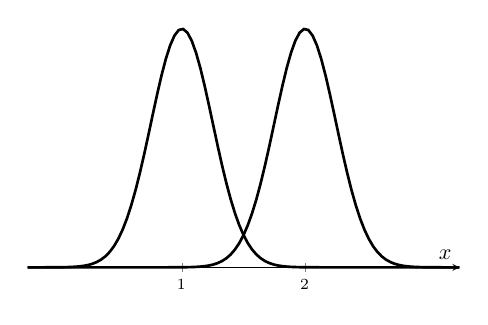
\begin{tikzpicture}[trim axis left, trim axis right, scale=0.8]
            \begin{axis}[
                domain = -4:10,
                ymin = -0.1,
                ymax = 0.5,
                samples = 101,
                axis y line=none,
                axis x line=middle,
                xtick = {1, 5},
                xticklabels = {$\m_1$, $\m_2$},
                xlabel = {$x$},
                legend cell align={left},
                legend pos=outer north east,
                ]
                \addplot[black, very thick] {1/(sqrt(2 * pi)) * e^(-0.5 * (x-1)^2)};
                \addplot[black, very thick] {1/(sqrt(2 * pi)) * e^(-0.5 * (x-5)^2)};
            \end{axis}
        \end{tikzpicture}
        \caption{Varying $\m$.}
    \end{figure}
\end{minipage}
\begin{minipage}{0.49\textwidth}
    \begin{figure}[H]\tikzsetnextfilename{431}
        \centering
        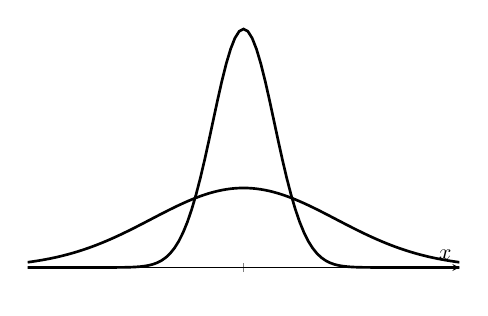
\begin{tikzpicture}[trim axis left, trim axis right, scale=0.8]
            \begin{axis}[
                domain = -4:10,
                ymin = -0.1,
                ymax = 0.5,
                samples = 101,
                axis y line=none,
                axis x line=middle,
                xtick = {3},
                xticklabels = {$\m$},
                xlabel = {$x$},
                legend cell align={left},
                legend pos=outer north east,
                ]
                \addplot[black, very thick] {1/(sqrt(2 * pi)) * e^(-0.5 * (x-3)^2)};
                \addplot[black, very thick] {1/(3 * sqrt(2 * pi)) * e^(-0.5 * ((x-3)/3)^2)};
            \end{axis}
        \end{tikzpicture}
        \caption{Varying $\s$.}
    \end{figure}
\end{minipage}

\medskip

Increasing $\m$ has the same effect as translating the normal distribution curve in the positive $x$-direction. Meanwhile, increasing $\s$ has the effect of flattening the normal distribution curve, i.e. the area under the curve about $\m$ becomes less concentrated, or more dispersed.

In a normal distribution, about 68.3\%, 95.4\% and 99.7\% of the values of $x$ are expected to lie within $\pm 1$, $\pm 2$ and $\pm 3$ standard deviations from the mean of $X$ respectively.

Perhaps the most important property of the normal distribution is that the sum or difference of normal distributions is also a normal distribution.

\begin{proposition}
    If $X$ and $Y$ are two \emph{independent} random variables such that $X \sim \Normal{\m_1}{\s_1^2}$ and $Y \sim \Normal{\m_2}{\s_2^2}$, then their sum and differences also follow a normal distribution: \[aX + bY \sim \Normal{a \m_1 \pm b \m_2}{a^2 \s_1^2 + b^2 \s_2^2}.\]
\end{proposition}

\subsection{Standard Normal Distribution}

\begin{definition}
    A random variable $Z$ is said to follow a standard normal distribution if $Z \sim \Normal{0}{1}$, i.e. $Z$ has mean 0 and variance 1.
\end{definition}

Suppose $X \sim \Normal{\m}{\s^2}$. Then the random variable defined by $Z = (X - \m)/\s$ follows a standard normal distribution. The process of converting $X \sim \Normal{\m}{\s^2}$ into $Z \sim \Normal{0}{1}$ is known as \vocab{standardization} and can be viewed as a transformation on the normal curve of $X$.

Standardization is typically used to compare different random variables that follow normal distributions, such as test scores for different subjects.

\begin{definition}
    Let $X \sim \Normal{\m}{\s^2}$, and let $x$ be an observation of $X$. Then the normalized score of $x$, called a \vocab{$z$-score}, measures the position of a score from the mean where its distance from the mean is measured in standard deviations. Mathematically, \[z = \frac{x - \m}{\s}.\]
\end{definition}

As the definition suggests, the higher the $z$-score, the better $x$ is relative to its distribution. For instance, if $z = 1$, then $x$ is 1 standard deviation above the mean, while if $z = -2$, then $x$ is 2 standard deviations below the mean.

\begin{sample}
    In the final year examination, a student obtains a score of 70 for Chemistry and 65 for Mathematics. If the cohort's scores for Chemistry and Mathematics follows $\Normal{60}{10^2}$ and $\Normal{57}{4^2}$ respectively, which subject did the student do better in?
\end{sample}
\begin{sampans}
    Normalizing the student's Chemistry score, we get a $z$-score of \[z_1 = \frac{X - \m}{\s} = \frac{70 - 60}{10} = 1.\] Normalizing the student's Mathematics score, we get a $z$-score of \[z_2 = \frac{X - \m}{\s} = \frac{65 - 57}{4} = 2.\] We see that the student has a higher $z$-score for Mathematics than for Chemistry. Thus, even though the student obtained a higher score for Chemistry, he did better in Mathematics when compared against his peers.
\end{sampans}

The standard normal distribution is also used for various scoring systems, such as PSLE T-scores, IQ scores and SAT scores.

\subsection{Normal Distribution as an Approximation}

Previously, we saw how the binomial distribution, under certain conditions, could be approximated to the Poisson distribution. Similarly, the normal distribution can be used to approximate both the binomial and Poisson distributions when certain conditions are satisfied.\footnote{This is a consequence of the Central Limit Theorem, which we introduced earlier in the section.}

However, unlike the case of binomial to Poisson, which is a discrete-to-discrete approximation, approximately either the binomial or Poisson distribution to the normal distribution is a discrete-to-continuous change. We hence introduce the idea of a ``continuity correction''. Intuitively, what this means is that $\P{X = k}$ (in the discrete case) is taken to be $\P{k-0.5 < X < k + 0.5}$ (in the continuous case). For instance, $\P{X = 16} = \P{15.5 < X < 16.5}$, and $\P{2 < X \leq 20} = \P{2.5 < X < 20.5}$.

\subsubsection{Approximating the Binomial Distribution}

\begin{proposition}
    If $X \sim \Binom{n}{p}$ and $n$ is sufficiently large such that $\m = np > 5$ and $n(1-p) > 5$, then $X$ can be approximated by $\Normal{np}{npq}$, taking into account the continuity correction.
\end{proposition}

If $p$ is close to $0.5$, the binomial distribution is almost symmetrical. Thus, the approximation by a normal distribution (which is symmetrical) gets better as $p$ gets closer to $0.5$.

Consider the following figure, where $X \sim \Binom{15}{0.5}$. We can approximate the distribution $X$ with a normal distribution with mean $np = 7.5$ and variance $np(1-p) = 3.75$.

\begin{figure}[H]\tikzsetnextfilename{432}
\centering
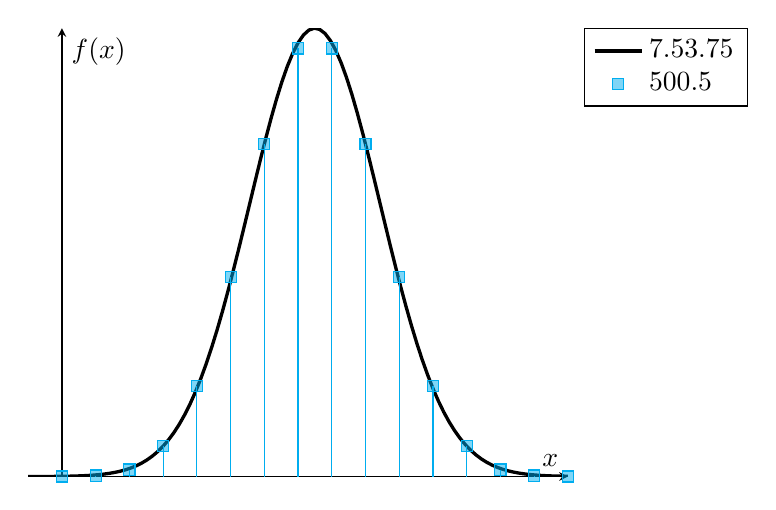
\begin{tikzpicture}
\begin{axis}[
    domain=-1:15,
    samples = 101,
    axis y line=middle,
    axis x line=middle,
    xtick = \empty,
    ytick = \empty,
    xlabel = {$x$},
    ylabel = {$f(x)$},
    legend cell align={left},
    legend pos=outer north east,
    ]

\addplot [black, very thick] {1/(1.94 * sqrt(2 * pi)) * e^(-0.5 * ((x-7.5)/1.94)^2)};
\addlegendentry{$\Normal{7.5}{3.75}$};

\addplot+[ycomb, domain=1:15, samples at={0,...,15}, cyan, fill opacity=0.5, mark options={cyan}]{15! / (x! * (15-x)!) * (0.5)^(15)};
\addlegendentry{$\Binom{50}{0.5}$};
\end{axis}
\end{tikzpicture}
\caption{Approximating the binomial distribution.}
\end{figure}

\subsubsection{Approximating the Poisson Distribution}

\begin{proposition}
    If $X \sim \Po{\l}$ such that $\l > 10$, then $X$ can be approximated by $\Normal{\l}{\l}$, taking into account the continuity correction.
\end{proposition}

\begin{figure}[H]\tikzsetnextfilename{433}
    \centering
    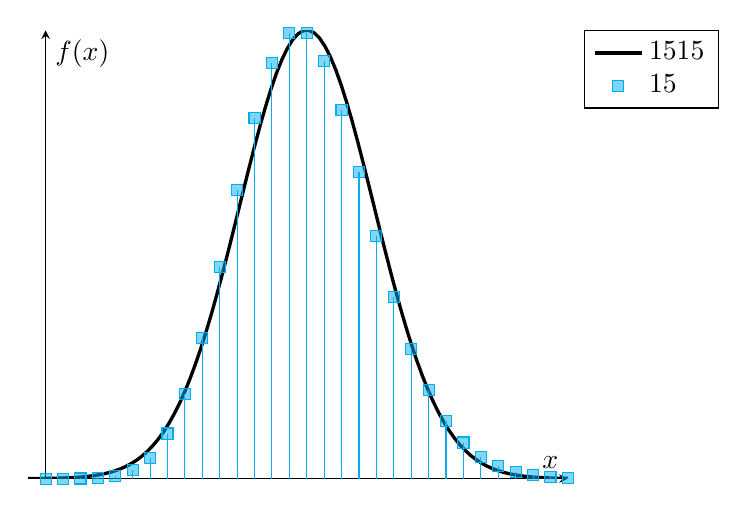
\begin{tikzpicture}
    \begin{axis}[
        domain=-1:30,
        samples = 101,
        axis y line=middle,
        axis x line=middle,
        xtick = \empty,
        ytick = \empty,
        xlabel = {$x$},
        ylabel = {$f(x)$},
        legend cell align={left},
        legend pos=outer north east,
        ]
    
    \addplot [black, very thick] {1/(3.87 * sqrt(2 * pi)) * e^(-0.5 * ((x-15)/3.87)^2)};
    \addlegendentry{$\Normal{15}{15}$};
    
    \addplot+[ycomb, domain=1:30, samples at={0,...,30}, cyan, fill opacity=0.5, mark options={cyan}]{(15)^x / x! * e^(-15)};
    \addlegendentry{$\Po{15}$};
    \end{axis}
    \end{tikzpicture}
    \caption{Approximating the Poisson distribution.}
\end{figure}